\section{Experiment}
To confirm NaaA widely work with machine learning tasks,
we confirm our method supervised learning tasks as well as reinforcement learning tasks.
As supervised learning tasks, we use typical machine learning tasks such as image classification
using MNIST, CIFER-10 and SVHN.

As reinforcement tasks, we confirm single- and multi-agent environment.
The single-agent environment is from OpenAI gym.
We confirm the result with a simple reinforcement task, CartPole.
In multi-agent, we use ViZDoom, a 3D environment for reinforcement learning.

\subsection{Classification}
In classification task, we experiment our method with several standard datasets, MNIST, CIFER-10 and SVHN.
As comparison method, we compare baseline (vanilla feed-forward neural network) and DropConnect.
In hyperparemeter setting, we set $\epsilon = 0.2$, which means the agent randomly masks the weights in 0.2 of chance rate, 
and playing the auction game in 0.8 of chance rate.
Table \ref{tbl:result} shows our framework of NaaA complements drawback of DropConnect, 
which it completely randomly drops the weight, and does not considering implicit counterfactual return of units.

\subsection{Single-agent RL}
Next, we set the single-agent reinforcement learning task.
We used CartPole task from OpenAI gym with visual input.
In the setting, the agent need to balancing a pole with moving a cart.
There are a lot of unuseful information on the image, pruning the pixel is important issue.
The result shows that our method improves the standard RL,

\subsection{Multi-agent RL}
The additional feature of NaaA is credit assignment for reward distribution, 
meant that if the neural network divided into multiple agents, it works by playing auction game.
We confirm additional agents complements the main player, we used ViZDoom, an environment for Doom.
A player in Doom environment should seek in the map, and defeat the enemy.
ViZDoom provides several maps. So, we used it.

\subsubsection{Setup}
We used a scenario based on Defend the Center (DtC) provided by ViZDoom platform.
In DtC, players are placed in a center of a field of circle, and attack enemies which will come from the wall.
The setting of a game has has two players: a main player and a cameraman.
Though the main player can attack the enemy with bullets, 
the cameraman does not have the way to attack, and only scout for the enemy.
The action space for main player is the combination of \{ attack, turn left, turn right \}. That is total amount of action is $2^3 = 8$.
Cameraman has two possible actions \{ turn left, turn right \}.
Although, the players only can move the direction, they cannot move on the field.
The enemy will die if have the attack (bullet) from the main player once.
The amount of ammo is 26 as a default on an episode.
The main player will die if have attacks from the enemy, and the health become 0.
The cameraman won't die if have attacks from the enemy.
The episode will terminate when the maim player dies, or 525 steps elapsed.

DtC is standard scenario which prepared by ViZDoom platform.
In DtC, up to 5 enemies appear can exists in the same time. 
The main player will receive reward every time defeat the enemy.
After the enemy dies, the player receives 1, if the player die, he receives -1.

\subsubsection{Model}
We compared three models: one is the proposed method, and the remaining are comparing target.

{\em Baseline} DQN without communication. The main player learns standard DQN with vision which he watching.
Since the cameraman does not learn, he continues to move randomly.

{\em Comm} DQN with communication. The main player learns DQN with two visions of him and cameraman.
The communication vector is learnt with a feed-forward neural network .  The method is inspired by CommNet.

{\em NaaA} The proposed method. The main player learns DQN with two visions of him and cameraman.
The transmission of reward and communication will be performed by proposed method.

\subsubsection{Results}
The training is performed in 10 million steps.
The figure \ref{fig:learning_curve} illustrates that our model NaaA outperforms CommNet.
The improvement is achieved by distribution of rewards and adaptive dropout.
We confirmed the cameraman see the enemy through an episode.
This can interpret as the cameraman reports the position of enemy.
Not only the enemy, the cameraman sees the behind of main player in several times.
This action enables the cameraman to observes attacks from the enemy with grabbing relative position.

For further interpretation of the result, 
we illustrates the visualization of revenue which the agent earned in Figure \ref{fig:vis} as a heatmap.
The background picture is screen in Doom taken in the moment which the filter in CNN is mostly activated.
Figure \ref{fig:vis} (a) shows that the agent see the top and center of screen.
The center corresponds to position that enemy appears far away, 
and the top corresponds to position that enemy come closer.
Figure \ref{fig:vis} (b) shows that the agent see the pistol.

\begin{figure*}[t]
\centering
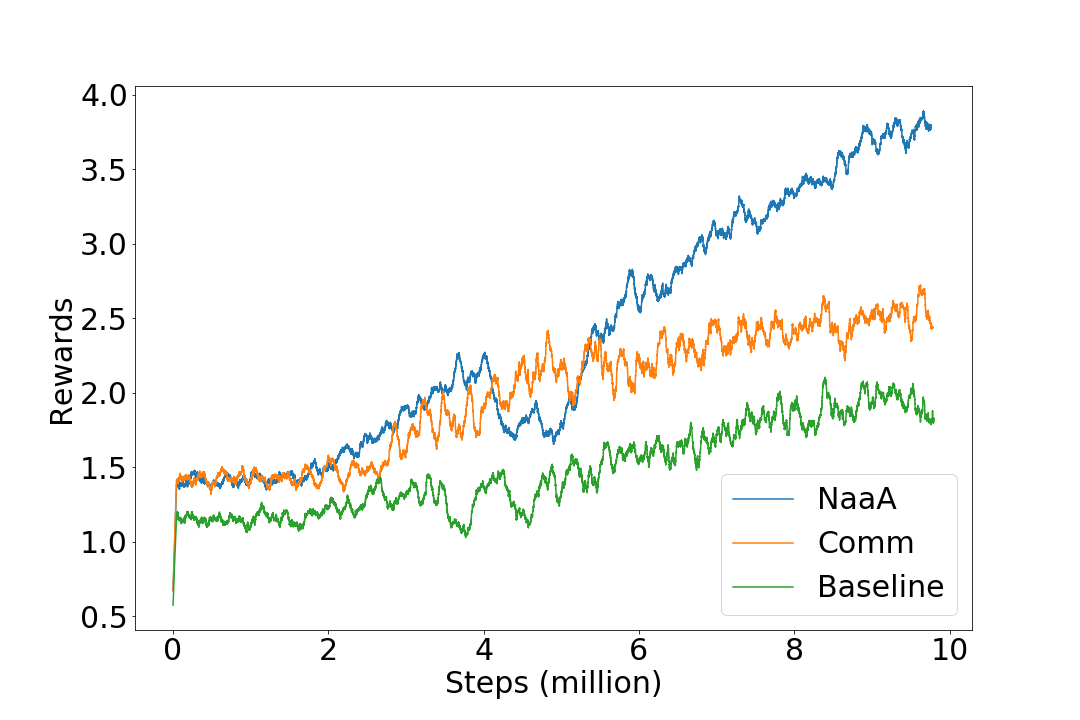
\includegraphics[width=3in]{img/learning_curve.eps}
\caption{
Learning curve for the multi-agent task of VizDoom. 
Our method based on NaaA outperforms other two methods, baseline and CommNet \citep{sukhbaatar2016learning}.
}
\label{fig:learning_curve}
\end{figure*}

\begin{figure*}[t]
\centering
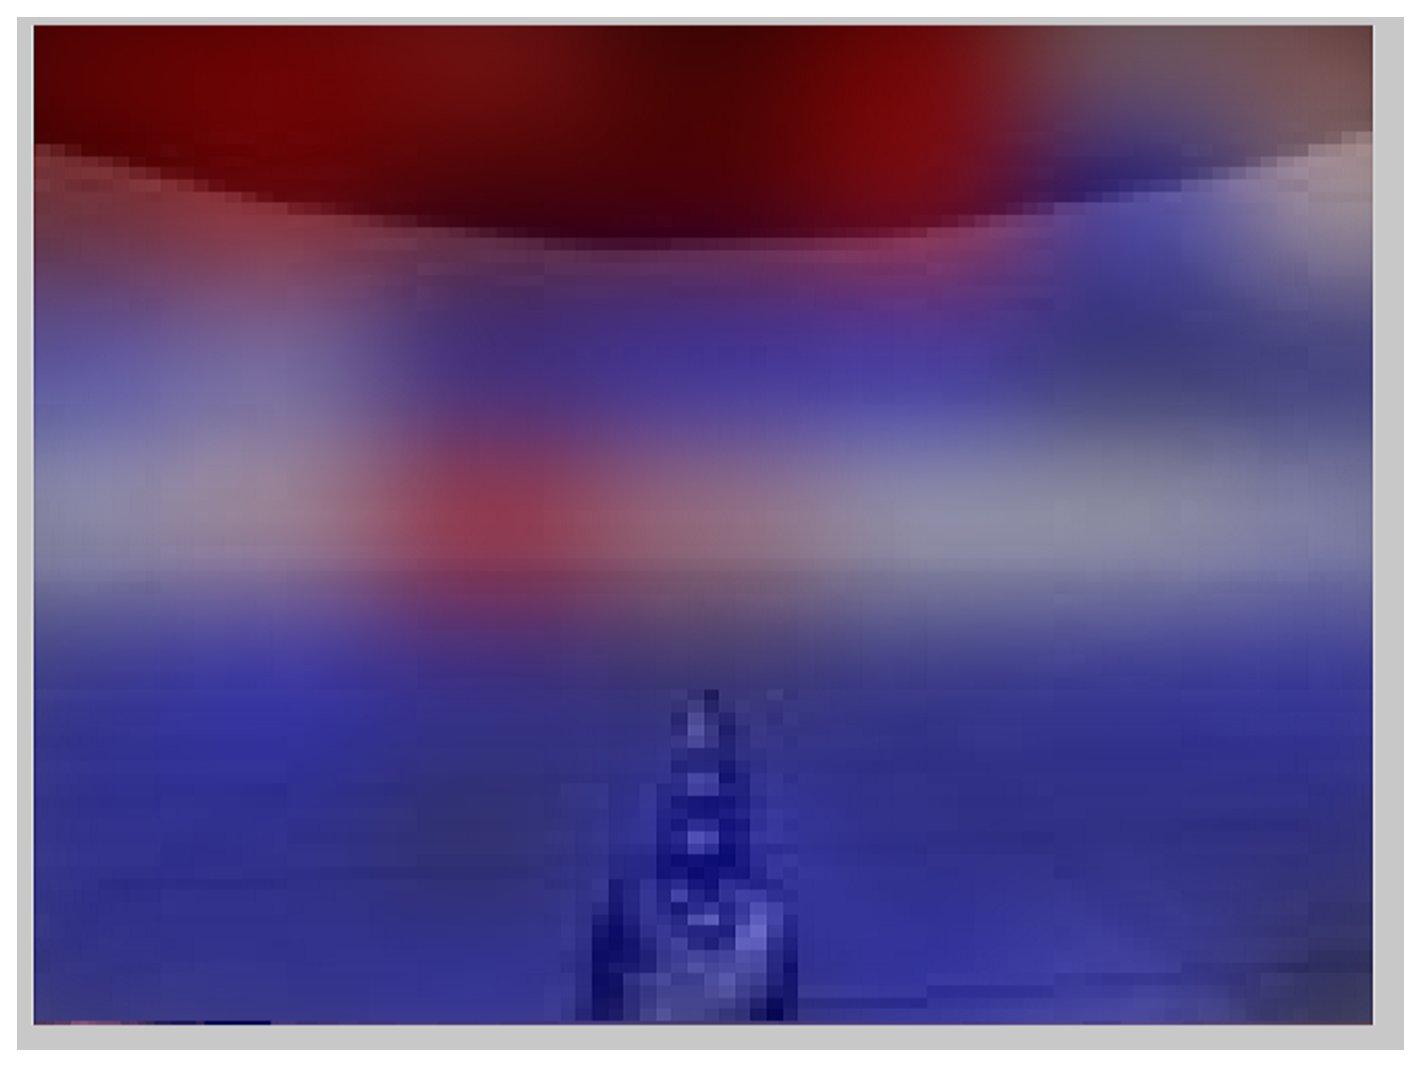
\includegraphics[width=2.5in]{img/vis1.eps}
\centering
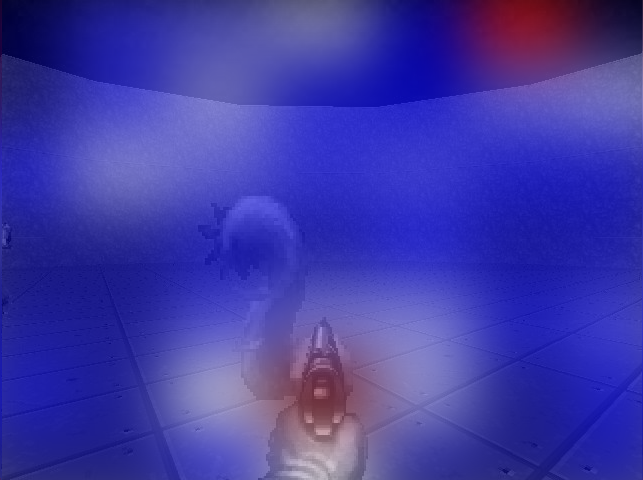
\includegraphics[width=2.5in]{img/vis2.eps}

(a)
\,\, \,\, \,\, \,\, \,\, \,\, \,\, \,\, \,\, \,\, \,\, \,\, \,\, \,\, \,\, \,\, \,\, \,\, \,\,
(b)
\caption{
Reward visualization tells us what the cameraman sees. 
(a) cameraman sees the point which enemy appear and come closer.
(b) cameraman sees the pistol.
}
\label{fig:vis}
\end{figure*}


%訓練は1000万ステップ行われた。
%TODO: 1.スコアが高いことを言う。2.潜在変数の値段や、シグナルの活性化を見る。
